\chapter{Introduction}
\label{sec:introduction}

\section{Motivation}

Computer-aided applications play a crucial role in engineering. Since the 1950s, many engineering projects rely on software to execute simulations and analysis of a wide variety of domains. Engineering (Civil, Mechanical, Electrical) has a heavy focus on mathematical models, time optimisations and new applications for modern techniques. Nevertheless, in many situations, engineers of these domains do not spend much time investigating a vital tool at the development of computer software: programming languages. 

One of the earliest and most concise definitions of programming languages comes from \cite{sammet1972programming}. 
\begin{quote}
"[A Programming Language] is considered to be a set of characters and rules for combining them which have the following characteristics: (1) machine code knowledge is unnecessary; (2) there is good potential for conversion to other computers; (3) there is an instruction explosion (from one to many); and (4) there is a notation which is closer to the original problem than assembly language would be".
\end{quote}


The core of software engineering for industrial applications started with the Assembly language, moving towards more structured languages like Fortran, Algol, Cobol, PL/I, Basic, Pascal, C, Smalltalk, Prolog, C++, Matlab, and more recently, Python, R and Java \cite{parker2012history}. However, it is possible to find a much broader spectrum of programming languages as illustrated in Figure \ref{histprog} (source \cite{ibmpl}).

\begin{figure}[H]
   \centering
   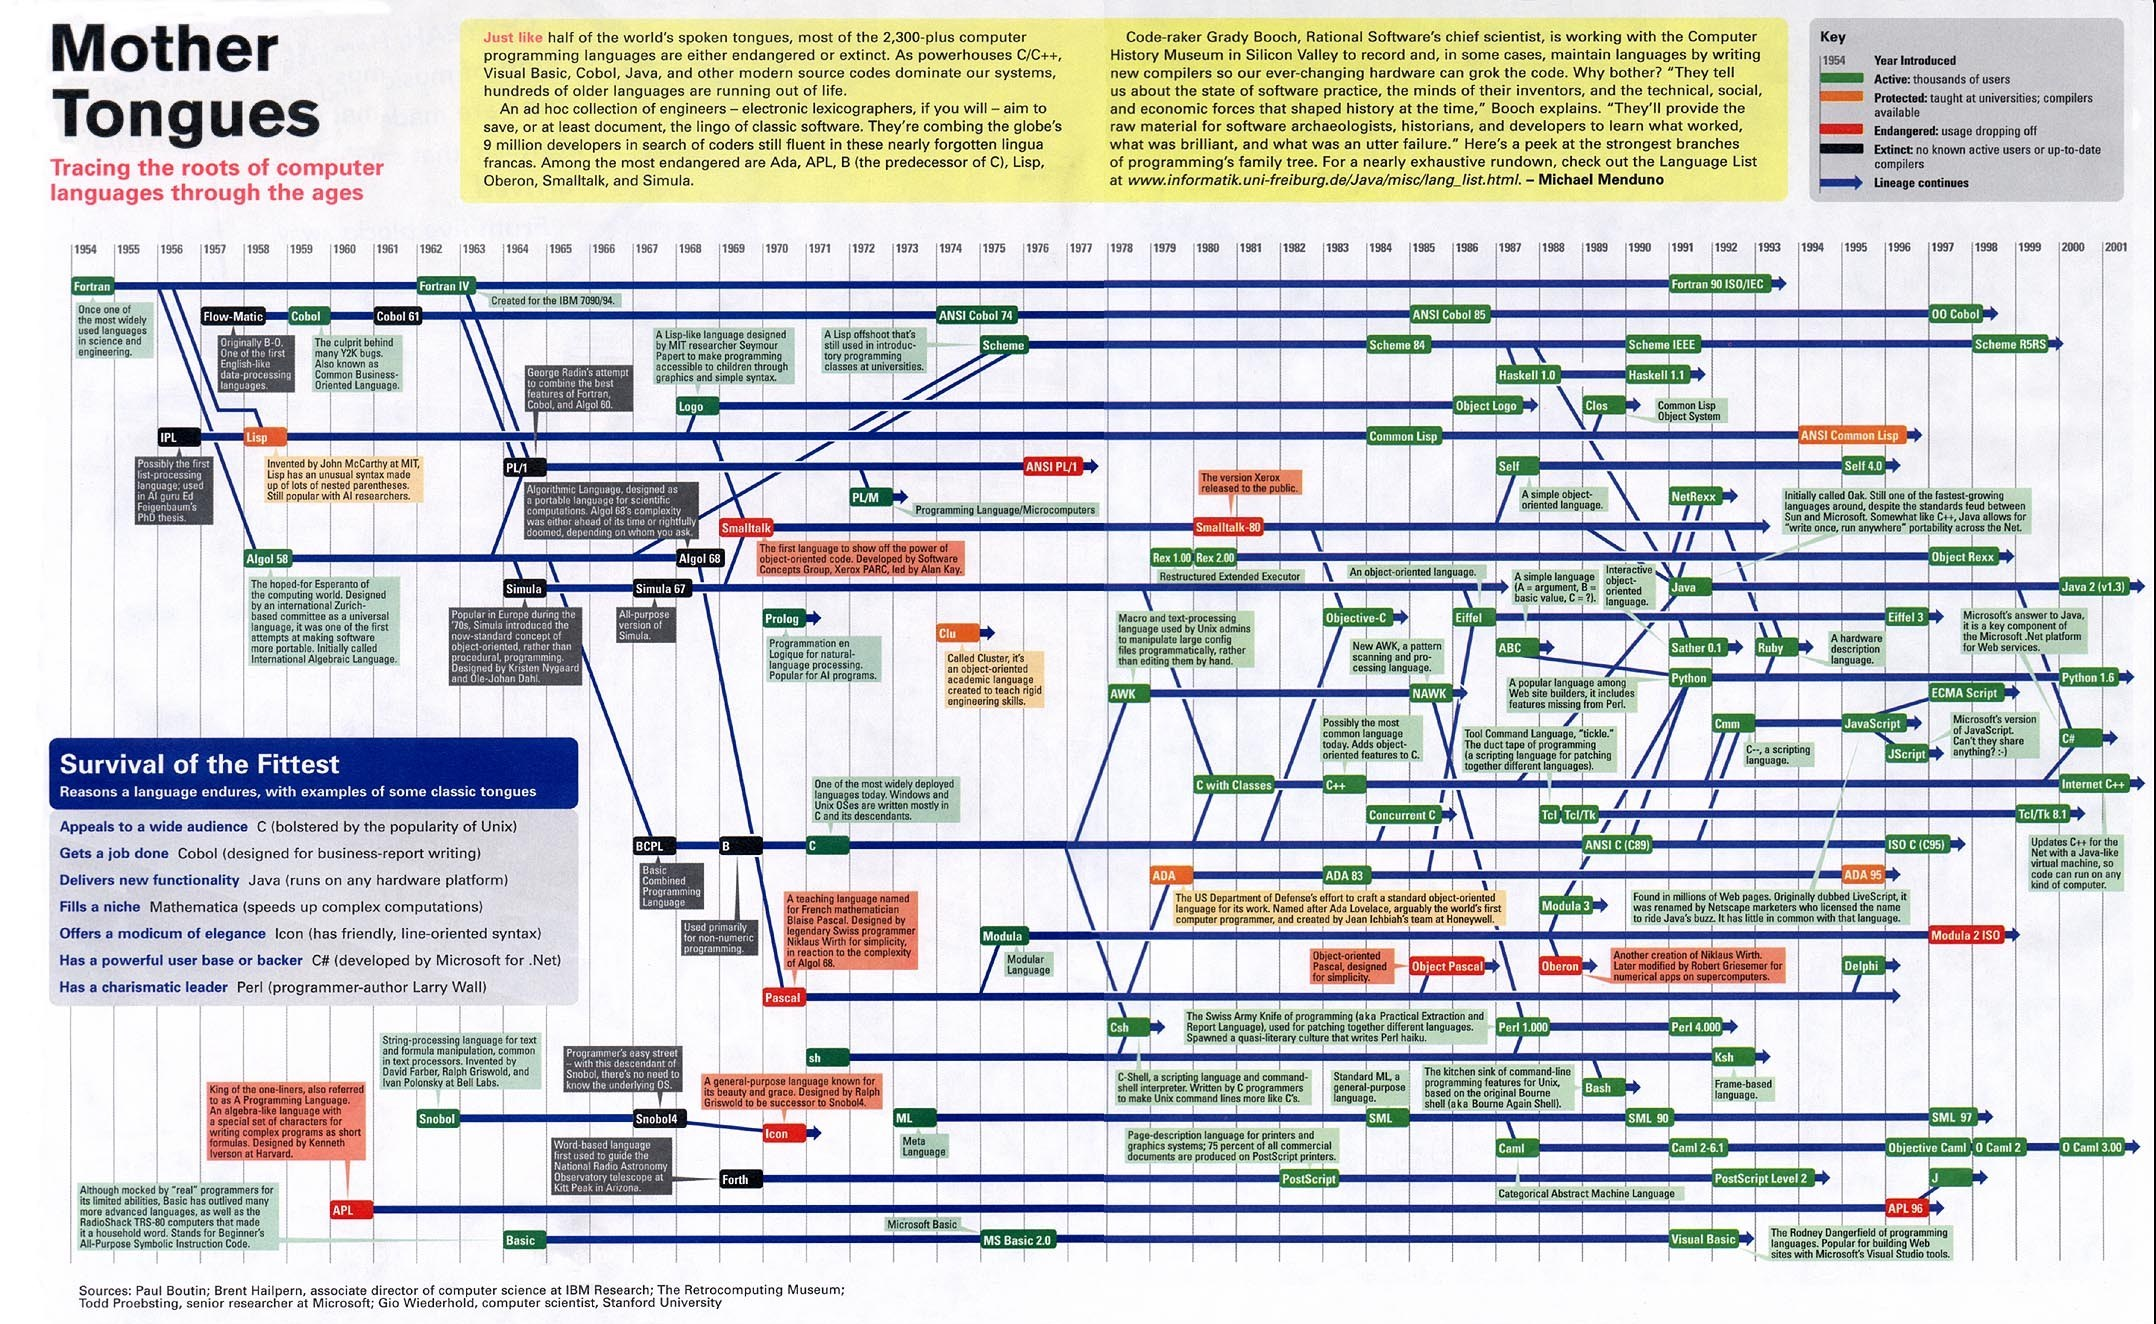
\includegraphics[angle=90,origin=c,width=0.95\textwidth]{img/histprog.jpeg}
   \caption{Programming languages history summary}
   \label{histprog}
\end{figure}


Programming languages itself is a dense topic, branching into compilers, static analysis, program synthesis, proofs, concurrency, type theory, logic and many others. Programming languages also have different paradigms \cite{felleisen2018design}. Historically speaking, the industry has been adopting procedural and \textbf{imperative} styles during the majority of the time.

\textbf{Imperative programming} is a paradigm that describes computation as statements - they can modify the state of the program. These statements focus on how they should solve the problem proposed in the algorithm, requiring a detailed instruction guide to perform.

There are different programming paradigms apart from the imperative style. Some languages follow the \textbf{Functional programming} paradigm - "they are descriptive rather than imperative, have no assignment command and no explicit flow of control - subcomputations are ordered only partially, by data dependency"\cite{turner2006church}. The principal component in this alternative paradigm is the application of a function to its arguments, not the computation of statements.   


\section{Research goals}
\label{rgoals}

This work proposes the adoption of the functional programming paradigm with a functional programming language to build a simple program reproducing a well-known algorithm for electromagnetic transient analysis of simple electrical circuits. This baseline algorithm uses a didactic program, developed in the MatLab plataform, by students at UNIFEI and UBC (see \cite{thtaoctave}). It aims to answer the following questions:



\begin{enumerate}
  \item What are the benefits of using a functional programming language? Will the development process be more intuitive? Will it be possible to apply all the functional programming concepts directly into the application domain? 
  \item What will be the differences with respect to the code base? Will it be shorter or longer? Will it produce a readable code?
  \item What will be the technical challenges? Functional programming is becoming more popular in the industry only in recent years, so there are not many documents and articles available to report challenges during the development process of engineering applications.
  \item How and why "functional languages are associated with fewer defects than either procedural or scripting languages"\cite{ray2014large}?
\end{enumerate}

The development of the Haskell application will answers the questions previously proposed.

Some of the complementary goals of this project are listed below.

\begin{itemize}
  \item Create an open-source implementation of a project using a real-world engineering application (electromagnetic transients) applying functional programming. There are not many projects in electrical engineering using this paradigm and this work can be a basic reference project for future research on similar topics.
  \item A software developer of electrical engineering applications should care about the tools he/she adopts. The programming language chosen is one of the main tools of the project. The selection of an inappropriate tool leads to bugs and unwanted behaviour. The correctness of the program also relies on the programming language. A professional software engineer will consider this matter when delivering a project.
\end{itemize}

\section{Relevance}

The future of engineering applications is strictly connected to advances in computer science and software development. Still, these two areas are mostly treated as entirely separate domains. This work aims to build a bridge between programming languages (with a case study on functional programming) and electrical engineering (with electromagnetic transient analysis).

The domain of programming languages research is vast. Analysing the use of functional programming for electrical engineering applications is just a starting point. This work is relevant because it can open doors for several future outputs, such as type analysis focused on the most common engineering models, formal verification of algorithms (increasing the reliability of the delivered software), and so on. Expanding this analysis to a field called Type Theory may lead to exciting results - would it be possible to guarantee that the written algorithm is mathematically equivalent to the engineering model? There are not many publications in this domain yet. Functional programming is the entry point for a more in-depth analysis of this matter.

\section{Methodology}

After a literature review on functional programming, Haskell (the functional language chosen to be the primary tool of this work) and existing applications, a working software containing the proof of concept (PoC) will be delivered and it will be publicly accessible on Github (a Git repository hosting service with free plans).

Once the PoC is done, its results will be compared with the ones produced by Matlab version, validating if the algorithm produces values at least similar to the ones produced by the Matlab version. A comparison between code paradigms will follow the numerical results.

Octave (an open-source implementation of Matlab) is used to run the simulations from the imperative implementation; Stack\cite{stack} and Cabal\cite{cabal} are used with GHC to compile and run the Haskell version. 

\section{Chapters Overview}

Chapter \ref{ch:etr} gives an overview of the Nodal Analysis in Electromagnetic Transient Analysis, as well as a historical context of the software build for this domain, both in industry and in academia.

Chapter \ref{fp} presents the most important concepts of functional programming. It will provide the reader with conceptual examples and possible applications. It uses the actual code from the Haskell program developed in this work.

Chapter \ref{haskell} applies the functional programming concepts described in the previous chapter to the Haskell language, providing a rich set of practical applications in the language. Haskell is not the only functional language available; there are others like OCaml, SML, Racket. Two separates chapters were kept in order to emphasise that learning functional programming is different from learning Haskell (although it is a necessary to know both for delivering good quality software and the results of this work).

Chapter \ref{implhs} provides a thorough explanation of the Haskell application. In every section of this chapter, there is a recap of the main algorithm for electromagnetic transient analysis, a walk-through the Haskell code and comparisons with the original didactic program developed in MatLab.

Chapter \ref{results} presents the results of the implementation, numerically comparing the values obtained from complete simulations in both versions, Haskell and Matlab. It then compares the development process for both of the paradigms, functional and imperative.

Chapter \ref{conclusions} answers the questions proposed at \ref{rgoals}. It also provides an extensive list of future work and a contribution guide for researches interested in the topic.
 
% Future work is also reported on the appendices. They provide the reader with an introduction to Lambda-calculus (\ref{sec:lc}), logic (\ref{sec:logic}) and type analysis (\ref{sec:proofs}).






